\section{Momento angolare}
%---------------------------------------------------------------------------
Il momento angolare è una grandezza molto importante in fisica, esso è
definito come il prodotto vettoriale tra il raggio vettore ed il vettore
impulso. È analogo alla quantità di moto, in quanto esprime un
concetto di resistenza non al cambio di velocità lineare come nel caso
dell'impulso, ma al cambiamento dello stato di rotazione di un corpo.
Infatti se un corpo ha un momento angolare costante nel tempo, allora si
muove di moto circolare uniforme. Mentre se il momento angolare varia nel
tempo, esisterà un'accelerazione angolare.

\begin{equation}
    \boxed{\vec L = \vec r \times \vec p = \vec r \times m\vec v}
\label{eq:momentum:L_def}
\end{equation}
\\
È importante ricordare che il momento angolare è uno pseudo-vettore in quanto
ha una forma diversa in base al polo rispetto al quale viene calcolato.
Ad esempio se trasliamo l'origine degli assi $O$ in $O'$, come mostrato in
figura (\ref{fig:momentum:pole_change}), otterremo che:

\begin{equation}
    \vec L = \vec r \times \vec p\quad \quad \vec L' = \vec r '\times\vec p =
    \sx\vec r + \vec t\dx\times \vec p = \vec r \times \vec p + \vec t\times
    \vec p = \vec L + \vec t\times\vec p
\end{equation}
\\
Quindi traslando il polo otterremo una variazione del momento angolare che è
la seguente:

\begin{equation}
    \boxed{\vec L'-\vec L = \vec t\times\vec p}
\label{eg:momentum:L_pole_change}
\end{equation}
\begin{figure}[htbp]
    \begin{center}
        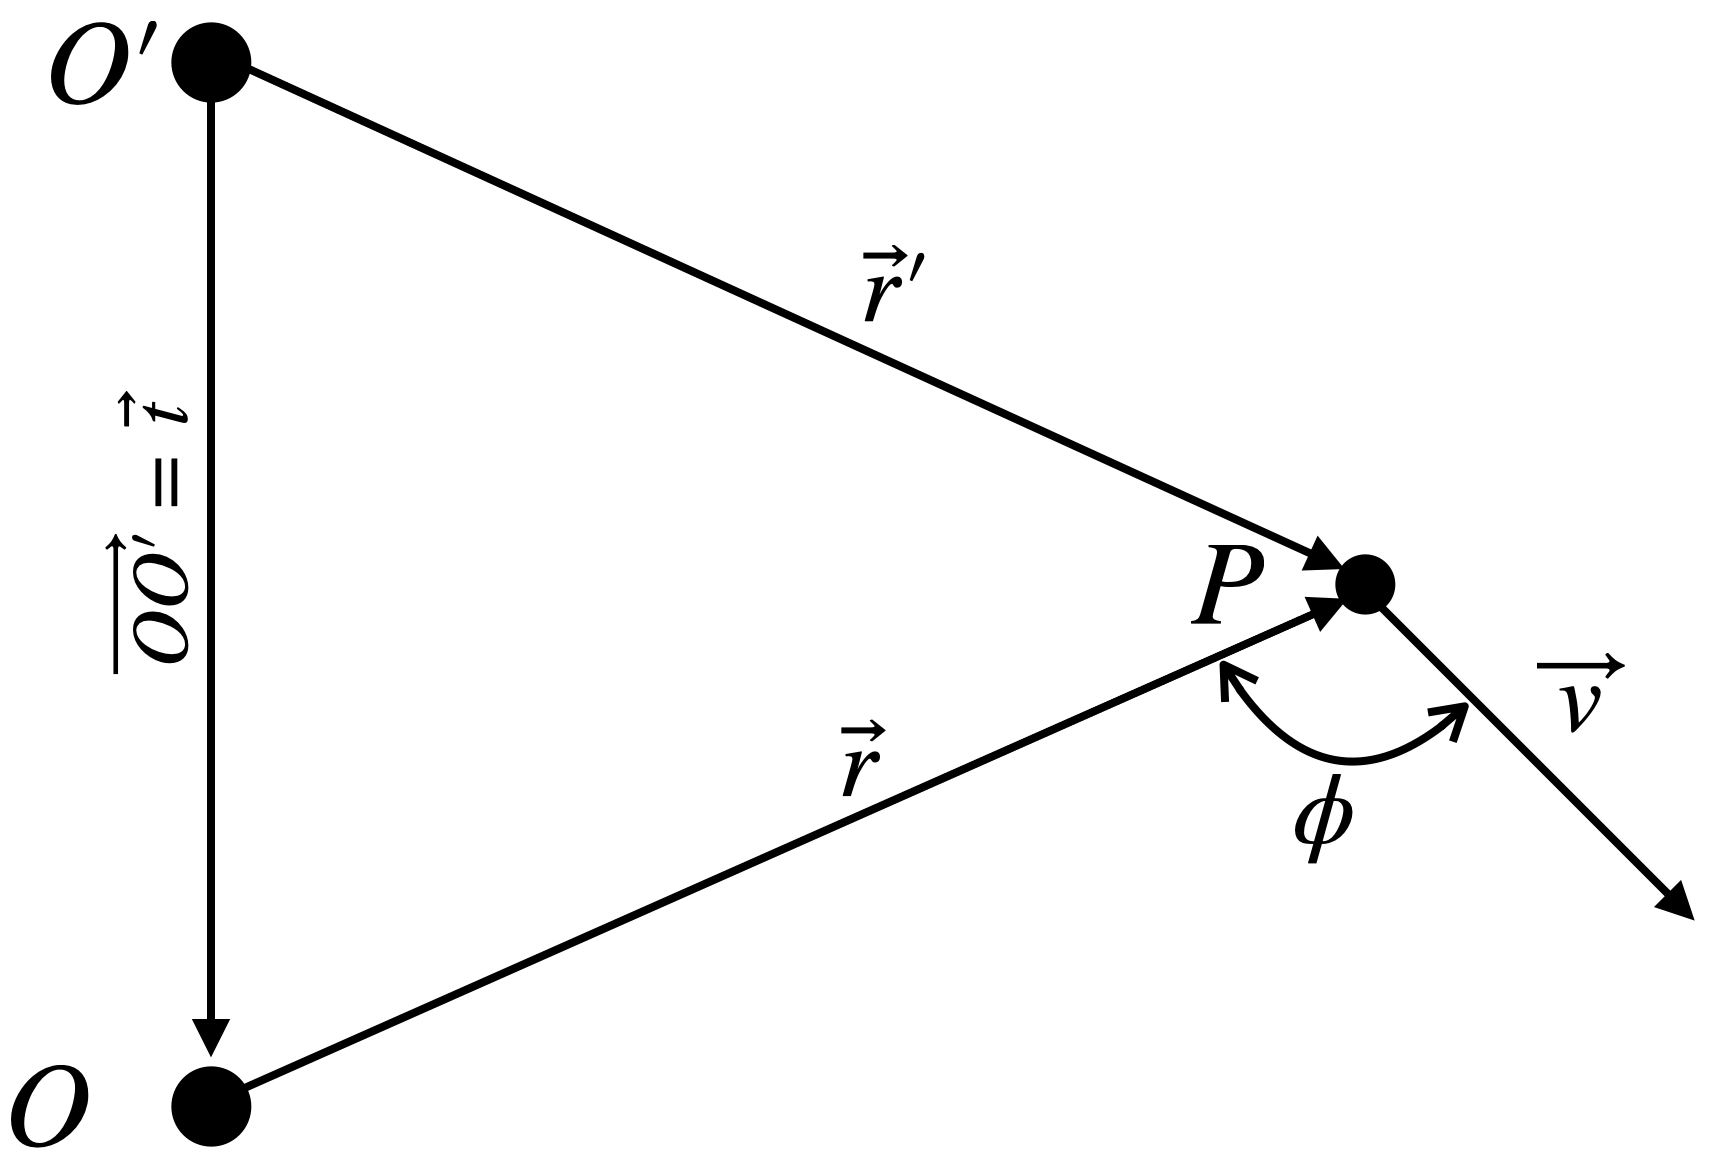
\includegraphics[width=10cm]{images/momang1.png}
        \caption{Schema dei vettori $\vec r$, $\vec r'$, $\vec v$ e $\vec t$,
        utilizzati per il calcolo del momento angolare rispetto ai poli $O$ ed
        $O'$.}
\label{fig:momentum:pole_change}
\end{center}
\end{figure}
\\
In coordinate polari possiamo scrivere la velocità come somma della sua
componente radiale e quella trasversa, ne segue che dato che la componente
radiale è parallela al raggio vettore, essa non da contributo al momento
angolare.

\begin{equation}
    \vec L = \vec r \times m\sx \vec v_r+\vec v_\phi\dx = \vec r \times m\vec v_\phi
\end{equation}
\\
Quindi dato che $\vec v_\phi = r\frac{d\phi}{dt}\hat\phi$ possiamo scrivere il modulo
del momento angolare di un punto materiale nel seguente modo:

\begin{equation}
    \boxed{L = mr^2\frac{d\phi}{dt} = I\omega}
\label{eq:momentum:l=Iw}
\end{equation}
\\
Dove abbiamo chiamato $I$ il momento d'inerzia. Il momento d'inerzia è un
analogo del termine di massa che compare nella definizione di impulso,
quindi come la massa esprime un concetto di resistenza alla variazione dello
stato di moto, il momento d'inerzia rappresenta lo stesso concetto, ma per
moti rotatori. Da notare dunque l'analogia in formule:
$\vec p$ con $\vec L$, $m$ con $I$ e $\vec v$ con $\vec \omega$.

\begin{equation}
\vec p = m\vec v \quad\quad \quad \vec L = I\vec\omega
\end{equation} 
\\
In questo caso il momento d'inerzia di un punto che ruota su una
circonferenza di raggio $r$ è pari ad $I = mr^2$. Vedremo poi in seguito,
nel capitolo sui corpo rigidi, come in realtà questo momento d'inerzia per
corpo estesi è una matrice, dunque in generale potremmo incontrare casi in
cui il momento angolare non è parallelo alla velocità angolare.

\section{Momento di una forza}
%---------------------------------------------------------------------------
In analogia con il momento angolare, il momento di una forza è definito dal
prodotto vettoriale tra il raggio vettore e la forza.

\begin{equation}
    \boxed{\vec M = \vec r \times \vec F}
\label{eq:momentum:M_def}
\end{equation}
\\
Partendo dalla definizione di momento angolare, si può effettuare la derivata
rispetto al tempo ottenendo infine la relazione che lega momento angolare e
momento delle forze.

\begin{equation}
    \vec L = \vec r \times \vec p \seg \frac{d\vec L}{dt} =
    \cancel{\vec v\times\vec p} + \vec r \times \frac{d\vec p}{dt} \seg
    \boxed{\vec M = \frac{d\vec L}{dt}}
\label{eq:momentum:M=dot_L}
\end{equation}

\subsection{Teorema dell'impulso angolare}
Analogamente a quanto fatto per il teorema dell'impulso, iniziamo integrando
l'equazione (\ref{eq:momentum:M=dot_L}).

\begin{equation}
    \vec M = \frac{d\vec L}{dt} \seg \int_0^\tau dt\frac{d\vec L}{dt} = \int_0^\tau dt \vec M \seg \Delta \vec L =\int_0^\tau dt \vec M 
\end{equation}

\begin{equation}
    \vec{M}_m = \frac1\tau\int_0^\tau dt \vec M = \frac{\Delta \vec L}{\tau}
\end{equation}

\subsection{Conservazione del momento angolare}
Differentemente da quanto succede con l'impulso, il momento angolare può essere
conservato non solo in assenza di momenti esterni applicati.
Considerando infatti un potenziale centrale tale per cui $U_{(\vec x)} = U_{(r)}$
ovvero dipendente solo dal modulo del vettore $\vec x$, avremo che:

\begin{equation}
    \vec F = -\vec\nabla U_{(r)} = -\frac{dU}{dr}\vec\nabla r = -U'_{(r)}\hat r
\end{equation}
\\
La forza ha solo componente radiale, quindi può essere uscente o entrante da un
punto, chiamato centro della forza. Ne segue che:

\begin{equation}
    \frac{d\vec L}{dt} = \vec r\times\frac{d\vec p}{dt} = -U'_{(r)}\vec r\times\hat r = 0
\end{equation}